\chapter{Reverse Engineering PuzzleScript}
\label{ch:puzzlescript}
In this chapter, we take steps to extract PuzzleScript's design from its implementation through reverse-engineering the JavaScript implementation. As we previously mentioned, the reason we need to reverse engineer PuzzleScript is that the existing implementations are not suitable for our research purposes. Therefore, we create our own. However, PuzzleScript does not have a complete design document we can use\footnote{\url{https://groups.google.com/g/puzzlescript/c/UBe9M8QP-rk}}. We need a design document because we do not want our implementation to have similar pitfalls as the official implementation.

% However, to create our own, rather than porting an existing implementation, we need to be able to implement the design but PuzzleScript does not have a complete design document. 

% The design document resulting from this step is one of the contributions of this project.

\section{Approach}
We create a comprehensive PuzzleScript design document by performing design recovery on the existing implementation by Lavelle. Design recovery in our case involves going through the codebase and observing the behavior of the implementation. We have access to the codebase through the public GitHub repository and we can access the deployed implementation on the PuzzleScript website\footnote{\url{https://www.puzzlescript.net/editor.html}}.

Investigating PuzzleScript's codebase presents challenges. JavaScript is dynamically typed, which means that the type of variables and function returns is not guaranteed. For instance, the code \texttt{a + b} could be adding two integers together or concatenating two strings. The only way of guaranteeing either outcome is to run the code and observe it. We can use context clues such as comments and variable names in the early stages but validation requires the code to be observed during runtime. Comments are sparse in PuzzleScript's codebase and the code density is high. As a result, reverse engineering the design of the codebase is challenging. Recovering the design also relies on the software engineer knowledge of that specific language. We complement our approach by observing the program during runtime. We do this by subjecting the system under study to various inputs to observe its behavior. We combine both approaches to create the design document.

Part of PuzzleScript's design is documented in the bachelor thesis by Vermuelen\cite{vermeulenautomated}. Their thesis breaks down the design of PuzzleScript and implements that design using Rascal's Syntax Definition. This is similar to our approach, however, their design document and implementation are incomplete. Their goal is to generate code from keywords and their implementation serves that purpose. Our goal is to parse every PuzzleScript game in existence using a new  grammar that can be reused in future prototypes. As such, we need a design document that is more comprehensive and documents PuzzleScript's many corner cases.


\section{PuzzleScript's Design}
In this section, we describe the results of our reverse engineering. We frequently reference the PuzzleScript user manual\footnote{\url{https://www.puzzlescript.net/Documentation/prelude.html}}. The user documentation focuses on the specifics of games. We instead focus on the general syntax structure of PuzzleScript and on the contextual constraint that can be used for creating a static analyzer. We aim to provide a document that makes it easier to parse PuzzleScript while the user guide provides specific implementation details.

\subsection{General}
A PuzzleScript file stores the contents of exactly one \emph{game}. Anything within that file is considered content for that game and that game only. There exists no way of splitting a game into multiple files or storing more than one game into a single file.

A \emph{game} consists of a \emph{prelude} and multiple \emph{sections}. Sections consist of a header which is the name of the section between two optional lines of equal (=) sign. Sections are delimited by either two headers or a header and the end of the file. In the JavaScript implementation, these sections must be in a specific order but from a design perspective, there is no inherent need for a specific order. However, "define before use" is a natural policy of programming and PuzzleScript may rely on that. The grammar of a section's content depends on the section itself. PuzzleScript is a context-sensitive grammar. The rules of syntax apply differently based on the context, in this case the context is the section. The order of the sections is as follows:
\begin{itemize}
    \item Objects: Defines all objects to be used in the game
    \item Legend: Create shorthand links between symbols and objects to allow properties, aggregation of objects, and tilemap creation.
    \item Sounds: Defines handlers to play sounds when certain events happen
    \item Layers: How objects interact with each other movement-wise, whether they can stack or if they collide
    \item Rules: How objects interact, what happens when certain items are next to each other or if a player tries to move into a certain item
    \item WinConditions: Defines victory conditions for the level
    \item Levels: List of tilemaps and messages that represent the different rooms the player will explore
\end{itemize}

\emph{Comments} in PuzzleScript are delimited by parenthesis (\emph{()}) and can be placed anywhere. It is unclear whether that is a conscious decision or simply a byproduct of the fact that the engine strips all comments before compiling the game.

\subsection{Prelude}
A game's \emph{Prelude} consists of all the lines before the first section. Each line consists of one or two tokens: a \emph{keyword} and a \emph{value}. These pairs allow the developer to modify how the engine works and the visual aspect of the game. Certain keywords do not require a value, they simply need to appear in the prelude to have an effect. Values can be a string (a list of tokens displayed literally), a numeral (int or float), or a member from an enumerator. A full list of possible prelude keywords and their values is documented in PuzzleScript's user guide\footnote{\url{https://www.puzzlescript.net/Documentation/prelude.html}}. 

\subsection{Objects}
\emph{Object} are the building blocks of PuzzleScript's games. They make up everything the player can see and interact with. They are used in rules to define game mechanics, they are used in conditions to define how the player achieves victory and they are used in levels to define what kind of challenges they present.

An object consists of a \emph{name}, an optional \emph{legend}, a list of \emph{colors} and an optional \emph{sprite}. The name and the legend are on the same line, the color list on its own line, and the sprite is a 5x5 tilemap. Colors are either an HTML color code or a color keyword from the selected palette. The color palette available is decided by the developer in the prelude from a wide range. The sprite is a 5x5 tilemap of where the \texttt{.} represent a transparent pixel and numbers from \texttt{0-9} represent a colored pixel based on the index of the colored list. As can be seen in Figure \ref{fig:object_code}, \texttt{0} represents blue because it is the first color in the list of colors defined for that object.

\begin{figure}
    \centering
    \begin{lstlisting}[language=PuzzleScript, xleftmargin=2pt, , basicstyle=\ttfamily\footnotesize]
        Player
        black $\color{BurntOrange}orange$ $\color{darkgray}white$ $\color{blue}blue$
        $\color{black}.000.$
        $\color{black}.$$\color{BurntOrange}111$$\color{black}.$
        $\color{darkgray}22222$
        $\color{black}.$$\color{blue}333$$\color{black}.$
        $\color{black}.$$\color{blue}3$$\color{black}.$$\color{blue}3$$\color{black}.$
    \end{lstlisting}
    \caption{An object}
    \label{fig:object_code}
\end{figure}

The name and legend of the object can be almost any character, although choosing certain characters can be an issue in other sections. For example, naming an object using any of the directional arrows is technically allowed. However, that makes it impossible to use the object's name in a rule, where the directional arrows are reserved keywords. In other cases, using reserved keywords for objects still works but confuses the syntax highlighter and results in code that is difficult to read and understand to the programmer.

\subsection{Legend}
\emph{Legend} allow the developer to create shorthand references to one or more objects. A legend consists of a name and a sequence of references, separated by the equal (=) sign. The sequence of object references, either the object name or another legend, is separated by either 'and' or 'or'. Legend cannot mix separators and cannot reference a legend that makes use of the other separator. \emph{Properties} are object references separated by 'or'. Properties are used to reference multiple objects in the context of rules, victory conditions, and sound. \emph{Aggregates} are object references separated by 'and'. Aggregates represent objects that are stacked on top of each other. Aggregates are used to place multiple items on one pixel in Level tilemaps.

The name of the legend is subject to the same constraints as the name of an object. Aggregates and legends referencing a single object can be used on tilemaps as long as the legend name is only one character long. An example of the different combinations can be seen in Figure \ref{fig:legend_code}.

\begin{figure}
    \centering
    \begin{lstlisting}[language=PuzzleScript]
        Obstacle = Crate $\color{violet}or$ Wall
        P = Player
        O = Target $\color{violet}And$ Crate
    \end{lstlisting}
    \caption{Three legends}
    \label{fig:legend_code}
\end{figure}

\subsection{Sound}
\emph{Sounds} allow the game designer to define what sound to play in the case certain events happen. A sound consists of either a reference or a sound keyword (SFX[0-10]) followed by a list of conditions (moving left, stationary) and finally a sound seed. The editor generates a limited range of sound seeds for use within games. Examples of sounds are shown in Figure \ref{fig:sound_code} and the possible conditions are documented in PuzzleScript's user documentation\footnote{\url{https://www.puzzlescript.net/Documentation/sounds.html}}.

\begin{figure}
    \centering
    \begin{lstlisting}[language=PuzzleScript]
        player $\color{violet}move  up$ $\color{BurntOrange}142315$
        Player $\color{violet}Move  down$ $\color{BurntOrange}142313$
        Player $\color{violet}Move  right$ $\color{BurntOrange}142311$
        Crate $\color{violet}Move$ $\color{BurntOrange}412312$
        Player $\color{violet}CantMove up$ $\color{BurntOrange}41234$
        Crate $\color{violet}CantMove$ $\color{BurntOrange}41234$
        Crate $\color{violet}Create$ $\color{BurntOrange}41234123$
        $\color{violet}CloseMessage$ $\color{BurntOrange}1241234$
        Sfx0 $\color{BurntOrange}213424$
        Sfx3 $\color{BurntOrange}213424$
    \end{lstlisting}
    \caption{Combinations of keywords creating sound events}
    \label{fig:sound_code}
\end{figure}

\subsection{Collision Layers}
Layers are lines of sequences that consist of either object reference or properties separated by either an optional command (,) or a white space. The purpose of the section is to define whether objects can stack or if they collide. All objects defined in the game must be referenced in a layer. This restriction exists so that the developer does not accidentally spawn an object without collision. Referencing an object in multiple layers is technically allowed but not recommended and it raises a warning. Ignoring the warning can have unintended consequences such as layers being ignored, allowing for unintended movement. Figure \ref{fig:layer_code} illustrates an example of a layer.

% An example of a layer can be seen in Figure \ref{fig:layer_code}.

\begin{figure}
    \centering
    \begin{lstlisting}[language=PuzzleScript]
        Crate, Player, Wall
    \end{lstlisting}
    \caption{A Layer}
    \label{fig:layer_code}
\end{figure}

\subsection{Rules}
Rules are at the heart of PuzzleScript. A rule consists of a series of prefixes that affect the whole rule, a left-hand side \emph{"pattern"} and a right-hand side \emph{"replacement"}. 

The left-hand side must contain at least one \emph{rule part}, the right-hand side must contain 0 or exactly the same number of rule parts as the left-hand side.  Rule parts start with a \texttt{[} and end with a \texttt{]}. Within a rule part, there are a certain number of \emph{rule sections}, each rule part on the right must have the same number of sections as the equivalent rule part on the left. Sections of a rule part are separated by \texttt{|}. Each section consists of object references that can stack, and each object can have one \emph{modifier}. Modifiers allow checking for special matches such as moving objects or the absence of an object. Each section represents an adjacent cell, either vertical or horizontal. Rules can be marked as "late" which means they will run in a second phase after the player movement has been processed. More information on the rules and the modifiers can be found in PuzzleScript's user manual\footnote{\url{https://www.puzzlescript.net/Documentation/rules.html}}. Figure \ref{fig:rule_code} illustrates a few examples of Rules.

\begin{figure}
    \centering
    \begin{lstlisting}[language=PuzzleScript]
        [ $\color{violet}>$  Player | Crate ] $\color{BurntRed}->$ [  $\color{violet}>$  Player | $\color{violet}>$ Crate  ]
        $\color{violet}late$ [ Crate | Crate | Crate ] $\color{BurntRed}->$ [ | |]
    \end{lstlisting}
    \caption{A few Rules}
    \label{fig:rule_code}
\end{figure}

\subsection{Win Conditions}
\emph{WinCoditions} offer a simple way of creating victory conditions that determine when a player has completed  (or won) a level. If no conditions are defined, the player will be unable to win a level. If multiple conditions are defined then all of them must be true simultaneously for the player to win. A condition consists of a victory keyword, an object reference or a property, and an optional 'on' condition. An 'on' condition consists of the word 'on' and an object reference. Conditions check whether an object exists on the level (or does not exist). The 'on' condition further requires that the object referenced in the condition be on the same XY-coordinates as the object referenced in the 'on' condition.

Valid keywords for a condition are \texttt{Some}, \texttt{No} and \texttt{All}. A condition with the \texttt{Some} keyword becomes true if at least one of the objects referenced is present on the level. If the 'on' condition is defined, it becomes true if at least one of either object is stacked on the other. A condition with the \texttt{No} keyword becomes true if zero objects are present on the level. If the 'on' condition is defined, then it becomes true if zero of either object are stacked. A condition with the \texttt{All} keyword cannot be used without the 'on' condition being defined. With the 'on' condition defined it becomes true if all objects referenced in the 'on' condition are stacked with an object from the condition. A few examples of these conditions can be seen in Figure \ref{fig:conditions_code}

\begin{figure}
    \centering
    \begin{lstlisting}[language=PuzzleScript]
        $\color{violet}Some$ target $\color{violet}on$ crate
        $\color{violet}No$ Player
        $\color{violet}All$ oranges $\color{violet}on$ plates
    \end{lstlisting}
    \caption{Three win conditions}
    \label{fig:conditions_code}
\end{figure}

We note that the syntax of the "Object1 on Object2" syntax can be confusing, and perhaps even misleading. For example, in the case of \texttt{All Crate on Target} what this means is that there cannot be a target that is not on the same XY coordinate\footnote{We define "stacked" as being on the same XY coordinate as PuzzleScript does not require for a specific item to be on top, as such, an item can still be on another item even if that first item is actually under.} as a Crate. However, from a natural language point of view, one would assume the contrary, that each Crate must be on the same XY as a Target. This distinction is important when there is more of Object1 than of Object2. For example, if there are four Target and three Crate then the level is impossible to win.

\subsection{Levels}
The level section consists of a combination of any number of \emph{Levels} and \emph{Messages}.  A Level is a rectangular 2-D tilemap of variable width and height that consists of symbols representing one or more objects. Only one character long reference can be used, whether they are legend or object names. Aggregation can also be used in levels but not properties.

A Message is a single line consisting of the word 'message' followed by a string (multiple words). When the Level before the message is completed, the engine will display the message before moving on to the next level. Any number of messages can be defined in between two levels, before the first level or after the last level. An example of a Message and Level can be seen in Figure \ref{fig:level_code}.

\begin{figure}
    \centering
    \begin{lstlisting}[language=PuzzleScript]
        $\color{violet}message$ $\color{BurntOrange}Level 1: Beginnings$
    
        ####..
        #.O#..
        #..###
        #@P..#
        #..*.#
        #..###
        ####..
    \end{lstlisting}
    \caption{A message and a level}
    \label{fig:level_code}
\end{figure}

\section{Implementation of PuzzleScript}
Here we describe the design decision of the 'official' implementation of PuzzleScript written by the original developer, Stephen Lavelle, in JavaScript.

The JavaScript implementation of the PuzzleScript engine consists of three separate phases. First, the source code is \emph{parsed} and checked for validity. Second, the \emph{compiler} transforms the parsed code into JavaScript data structures. This also involved transforming rules into JavaScript functions using meta-programming. Further verification is conducted during compilation. Finally, the \emph{engine} runs the game and awaits player input.

The repository containing the source code for PuzzleScript consists of 27 files and adds up to over 15,000 lines of code calculated using \emph{cloc}\footnote{\url{http://cloc.sourceforge.net/}}. Most of the files are used to store code that provides features not directly tied to PuzzleScript's design such as Saving/Exporting games. Those files also contain code for features that are small parts of the design but require large implementations such as sounds. Three files are responsible for the phases we identified above and total 5820 lines of code. The files are: \begin{itemize}
    \item parser.js: 1065 lines, responsible for the Parsing phase.
    \item compiler.js: 2350 lines, responsible for the Compilation phase.
    \item engine.js: 2405 lines, responsible for the Engine phase.
\end{itemize}

The in-browser IDE, a vital part of the implementation, is implemented using CodeMirror. CodeMirror is a versatile library specifically made for editing code in-browser. The IDE provides comprehensive syntax coloring that adapts to its context. Pixels representing a color will appear as that color in the respective sprites that use them. Syntax coloring will fail if the syntax is incorrect. 

\begin{figure}[h]
    \centering
    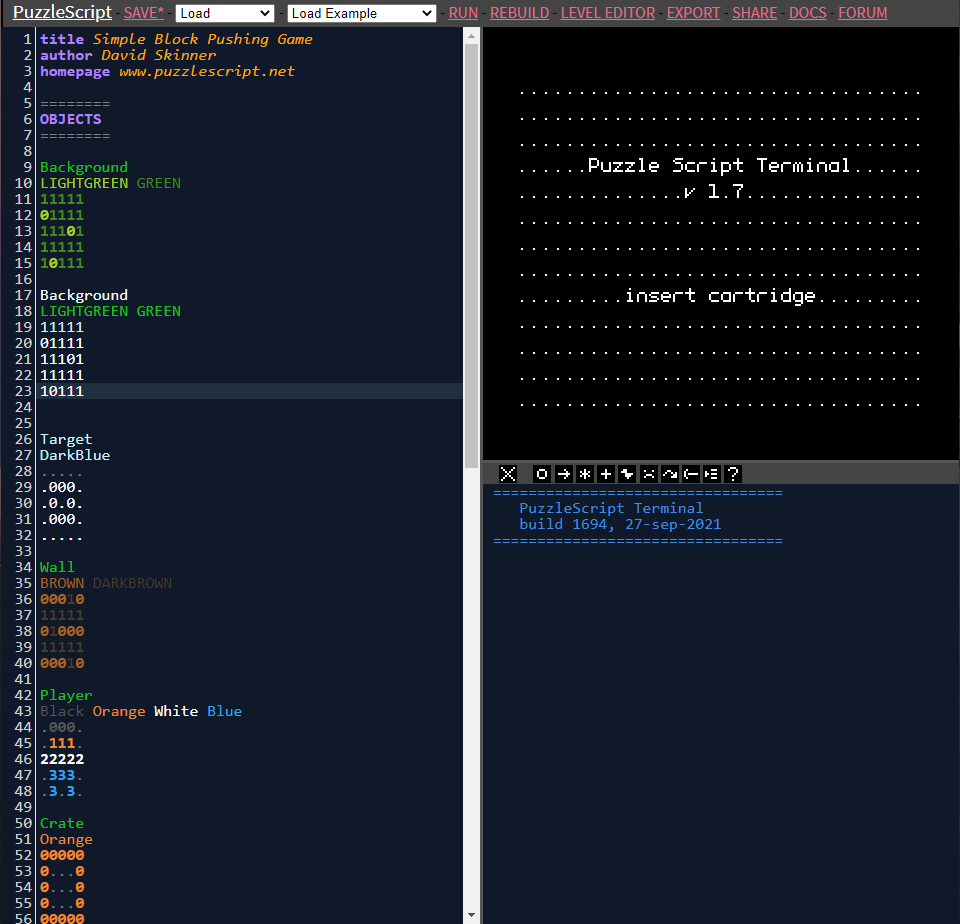
\includegraphics[width=1\textwidth]{images/PuzzleScript_IDE.png}
    \caption{PuzzleScript's browser IDE}
    \label{fig:browser_ide}
\end{figure}

Once the user presses "Run" the game compiles, errors appear in the bottom right and the title screen for the game appears in the top right. The top bar of the IDE provides additional options for sharing and exporting the game into a standalone application alongside helpful links for seeking support.

The implementation displays error messages as they are detected and aborts the compilation if a certain threshold is reached. The threshold is necessary because of the possibility of an error cascade. Without the threshold, a high number of ghost errors might be displayed. This would make it harder to fix the true issues. With the threshold, the developer is encouraged to address errors one by one, allowing the static checker to clear up any ghost errors. User inputs are context-sensitive. If the user presses an arrow key while focused on the editor, it will move their cursor text, if they do the same with a focus on the game, it will attempt to move their character. The IDE does not have a contextual right-click menu.

\section{Lessons Learned}
Here we analyze and discuss design decisions that complicate Puzzlescript's analysis. In particular, we discuss how language features lead to possibly complex situations when writing Puzzlescript due to 'dark corners' in the language semantics.

\subsection{Compilation}
PuzzleScript is an incredibly flexible language, both in design and through implementation. However, this flexibility includes corner cases in language semantics that make it hard to formalize the semantics.

For instance, PuzzleScript has section-specific reserved keywords. For instance, specifying the legend for an object as \textbf{]} is allowed. However, the trade-off is that the legend cannot be used to reference that object in the Rules section since \textbf{]} is a reserved keyword in the context of that section. This is made possible by the technical implementation of PuzzleScript's parse which is line-based and handcrafted. The flexibility of PuzzleScript's grammar places it in the category of context-sensitive grammars. Section-specific keywords are not a common design pattern. PuzzleScript's grammar leveraging that pattern poses a challenge to formalizing it.

% places PuzzleScript's grammar in the category of context-sensitive grammars.

% The question we pose now is whether or not this flexibility is worth the extra complexity. The flexibility makes it hard to create a formal grammar because section-specific keywords are not a common design pattern. 

The JavaScript implementation has tightly coupled compiler phases. This means that extending the codebase requires a full understanding of the entire process. There are no "general" functions that can be simply provided as a set of instructions for extensions. PuzzleScript does not provide an interface with helper functions but rather defines functions based on the current needs of the implementation.

\subsection{Intentional Ambiguities}
The design of PuzzleScript includes intentional ambiguities. Components can be defined in multiple ways with slight differences to their syntax. These multiple ways do not affect the behavior of the component but need to be handled by the parser. These variants of the syntax provide no real benefit and may even confuse the game designers. For instance, objects in collision layers are normally separated by a comma, making the formalization of the grammar appear simple. However, upon further inspection, we discover that a list of space-separated objects is also a valid line. This means that there are three possible separators for a collision layer that can be used interchangeable: 1) a comma with no whitespace; 2) a comma and a white space (in any order) and 3) just a whitespace.

% This means that the comma is no longer a separator but rather an optional token that may or may not separate objects. Three valid examples of the same layer can be seen in Figure \ref{fig:Layer Example}.

\begin{figure}[!t]
\begin{lstlisting}[language=PuzzleScript]
Crate,Player, Target
Crate Player Target
Crate, Player Target
\end{lstlisting}
\vspace*{-8pt}
\caption{Three examples of the same layer}
\label{fig:Layer Example}
\vspace*{-8pt}
\end{figure}

\subsection{Rule Semantics}
Rules, the heart of PuzzleScript, are complex to read and hard to maintain. The instructions of the rules are transformed into code which the compiler interprets as a JavaScript function. PuzzleScript's engine makes use of meta-programming as it generates the JavaScript code that represents the rules during runtime as a function. This means that a great part of the engine does not exist until runtime. Because JavaScript is dynamically typed, it is hard to understand what is being passed to these functions. 

In the JavaScript implementation, parsing is one of the two phases and is done simultaneously with error checking. This can very easily cause errors to cascade since any error also throws the parser off as can be seen in Figure \ref{fig:error_cascade}. The graphics and engine are similarly coupled, graphics are generated as rules are applied, and the objects have methods for generating graphics directly attached to them. Additionally, the error messages are duplicated throughout the process. This means that if a developer wants to change the wording of an error message, they need to go through the core files and modify every instance of the message.

\begin{figure}[!t]
    \centering
    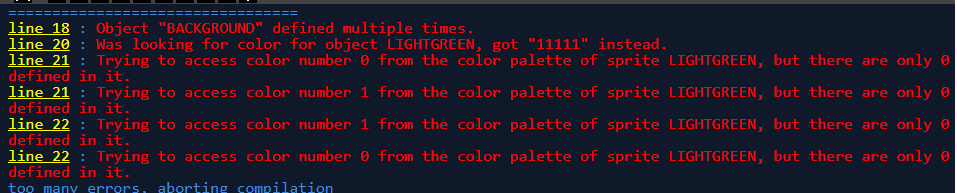
\includegraphics[width=1\textwidth]{images/Example_errors_current.png}
    \caption{A single error causes a cascade of ghost errors}
    \label{fig:error_cascade}
\end{figure}

\subsection{Interactive Development Environment}
The IDE itself is simple, offering syntax coloring, and printing errors. Its real power comes from the engine itself, which allows running games with great performance directly in the browser. When an error occurs, the syntax coloring breaks on the line where the error occurred. This allows for basic debugging but does not provide any information on what the error is. The debug console provides the necessary information to solve most errors. However, it usually only provides enough information to solve the first error encountered. Both of these aspects are functional and serve their purposes but have room for improvement.

\section{Conclusion}
We conclude that PuzzleScript is a complex language that appears simple to the users. The implementation focuses on performance and portability at the cost of extensibility and maintainability. This specific focus makes it hard to use to answer our research questions, as such, we design our own implementation.
